\documentclass[11pt]{article}

% ============================================================================
%  When Does Model Routing Help? A Native Router for LiteForge and a
%  Cross-Provider Cost-Quality Study
%  arXiv-style technical report
% ============================================================================
\usepackage[a4paper,margin=1in]{geometry}
\usepackage[T1]{fontenc}
\usepackage{lmodern}
\usepackage{microtype}
\usepackage{amsmath,amssymb}
\usepackage{booktabs}
\usepackage{tabularx}
\usepackage{graphicx}
\usepackage{xcolor}
\usepackage{enumitem}
\usepackage{caption}
\usepackage[numbers,sort&compress]{natbib}
\usepackage[hidelinks]{hyperref}
\definecolor{linkc}{HTML}{6D28D9}
\hypersetup{colorlinks=true, linkcolor=linkc, citecolor=linkc, urlcolor=linkc}

\newcommand{\rb}{\textsc{RouterBench}}
\newcommand{\rl}{\textsc{RouteLLM}}
\newcommand{\re}{\textsc{RouterEval}}
\newcommand{\code}[1]{\texttt{\small #1}}
% --- headline numbers (refresh as the cross-provider sweep completes) ---
\newcommand{\ROUTEREMBAPGR}{0.308}
\newcommand{\ROUTEREMBSAVED}{22.5}
\newcommand{\TASKHEADACC}{0.993}
\newcommand{\NPROV}{25}            % models measured in the cross-provider pool
\newcommand{\NPROMPTS}{290}        % cross-provider prompts per model
% --- Study 4: agentic (tau-bench airline, N=50, agent temp 0, 3 trials) ---
\newcommand{\TAUN}{50}
\newcommand{\TAUORACLE}{0.727}     % oracle-cascade quality, nemotron pool
\newcommand{\TAUSTRONG}{0.628}     % all-strong quality
\newcommand{\TAUSELFG}{0.613}      % self-consistency cascade, gemma pool
\newcommand{\TAUJUDGEREC}{0.60}    % best judge (glm-5.2) recall

\title{\textbf{When Does Model Routing Help?\\
A Native Router for LiteForge and a Cross-Provider Cost-Quality Study}}
\author{Sean Poyner \\ \small LiteForge}
\date{June 2026}

\begin{document}
\maketitle

\begin{abstract}
We present the model-routing subsystem of LiteForge, an open-source LLM SDK, and then
ask the question that decides whether such a subsystem is worth shipping: \emph{when
does routing actually beat simply picking a good cheap default?} The router has two
composable layers, a Layer-1 load balancer and a Layer-2 content/quality selector, and
its default selector is a lightweight logistic head over frozen \code{bge-m3}
embeddings. On \rb{}, a benchmark with a wide weak/strong quality gap, this head
recovers a real \ROUTEREMBSAVED\% of cost at iso-quality (APGR \ROUTEREMBAPGR{}), beating
trivial heuristics, utterance-similarity routing, a synthetic ``panel'' of tiny BERT
experts, and a from-scratch encoder. The cautionary finding comes next: on the actual
shipped pool of Claude tiers (haiku/sonnet/opus), the tiers are near-parity (haiku
reaches $\sim$95\% of sonnet; opus is Pareto-dominated), so \emph{the same router
recovers essentially nothing} (APGR $\approx 0$, CI spanning zero). Routing's value is
conditional on a recoverable quality gap. Pursuing the gap outward, we run a measured
cost-quality study over a cross-provider pool of \NPROV{} models (hosted APIs,
self-hosted, and open-weight models via Ollama Cloud) on quality-graded public
benchmarks with real gateway prices. Cheap hosted models (DeepSeek v4 Flash at
\$0.26/1M, Gemini 3.1 Flash-Lite at \$1.05/1M) deliver 95--96\% of Sonnet quality at
one to two orders of magnitude lower cost; the strongest open-weight models (gemma4:31b,
glm-5.2) reach $\sim$96\% of Sonnet but none beats it, and on published serverless rates they
are cheap too (gemma4:31b at \$0.78/1M undercuts Flash-Lite), so self-hosting is a residency
choice rather than a cost win. The practical lesson is that \emph{model
selection dominates clever routing} on the pools people actually deploy. Finally we push
into agentic tasks (tau-bench, real tools, \TAUN{} tasks, an LLM-simulated user): here even
a genuine capability gap is \emph{unroutable up front}, because difficulty is not legible
from the opening turn, and both our embedding head and a RouteLLM-style port score at or
below random. The frame that works is \emph{escalate-on-failure}: an oracle cascade
(\TAUORACLE{}) beats always-using-the-strongest tier (\TAUSTRONG{}), the best cheap trigger
is self-consistency (up to \TAUSELFG{}, $\sim$98\% of strong quality at $\sim$40\% of its
cost), and an LLM-judge verifier helps only when it is strong and calibrated (best recall
$\sim$\TAUJUDGEREC{}; small judges fail and none reach the oracle, since agentic failures are
silent). We release the full training, grading, and evaluation harness.
\end{abstract}

\section{Introduction}
Serving large language models forces a cost-quality trade-off: the strongest models are
many times more expensive than competent cheap ones, yet most queries do not need the
strongest model. \emph{Model routing} sends each query to an appropriate model. We
describe a production router built natively into LiteForge~\citep{liteforge} and, rather
than reporting only in-distribution numbers, subject it to three increasingly realistic
tests. The result reframes the problem: a router is only as valuable as the quality gap
it has to exploit, and on the pools that ship in practice that gap is often small enough
that the right move is to change the default model, not to route.

\paragraph{Contributions.}
\begin{enumerate}[leftmargin=1.4em,itemsep=2pt]
\item A two-layer router: LiteLLM-style load balancing~\citep{litellm} plus a pluggable
content/quality selector, reusing the SDK's transport unchanged. The default selector is
a linear head over frozen \code{bge-m3} embeddings that beats trivial heuristics,
utterance-similarity routing, and a synthetic panel at one embedding call plus a dot
product.
\item An honest, baseline-grounded benchmark study on \rb{} with bootstrap confidence
intervals, including a correction of two of our own earlier over-claims (a ``panel'' of
tiny experts and a native matrix-factorization port, both demoted).
\item The central negative result: on a real Claude haiku/sonnet/opus pool with
\emph{measured} quality and real gateway prices, the tiers are near-parity, so routing
recovers almost nothing. The \rb{} headline does not transfer to the shipped pool.
\item A measured cross-provider cost-quality study over \NPROV{} models spanning hosted
APIs, self-hosting, and open-weight models (via Ollama Cloud), quantifying where the
real savings live (cheap hosted defaults) and the open-weight quality ceiling
($\sim$96\% of Sonnet), with a build-vs-buy break-even analysis.
\end{enumerate}

\section{Related Work}
\rl{}~\citep{routellm} learns to route between a strong and weak model from preference
data, recommends matrix factorization, and reports up to 70\% cost reduction at fixed
MT-Bench quality, evaluated with the call-performance threshold (CPT) and average
performance gain recovered (APGR). \rb{}~\citep{routerbench} is the standard cost-quality
benchmark: over 30k prompts with each of 11 LLMs' correctness and cost plus oracle
labels. \re{}~\citep{routereval} frames routing as $m$-way classification at scale.
Semantic routers~\citep{semanticrouter} and LiteLLM's auto-router route by embedding
similarity to example utterances. All of this work assumes a meaningful strong/weak gap.
Our study's contribution to that literature is orthogonal and cautionary: we measure what
happens when the deployed pool does \emph{not} have a wide gap (near-parity Claude tiers)
and when the cheaper option lives at a different provider rather than a different tier of
the same family. In that regime the relevant decision is model \emph{selection} on a
measured cost-quality frontier, not a learned router.

\section{System Architecture}
\subsection{Two layers}
A request carries a logical model name (or the alias \code{auto}). Layer 2 (a
\code{ModelSelector}) returns a ranked list of model groups; Layer 1 load-balances within
the top group and falls back down the ranking on failure. The selector trait lives in the
Layer-1 module so the router can call it without a dependency cycle. Layer 1 mints a
per-deployment configuration and reuses the SDK's existing HTTP transport, so no
request-path rewrite was required. Strategies are weighted-shuffle, round-robin,
least-busy, and latency-based; failing deployments are cooled down after a configurable
number of consecutive failures.

\subsection{The default selector: an embedding head}
The default Layer-2 selector is a logistic head over a frozen \code{bge-m3} embedding of
the prompt, predicting whether the weak (cheap) model suffices; the route-to-strong
propensity is $1-\hat P(\text{weak correct})$. The cost is one embedding call plus a dot
product. A companion task head over the same embedding classifies qa/code/math for
code-aware capability routing. We also implemented, and then \emph{demoted}, two
components we initially over-credited: a four-expert ``panel'' of \code{bert-tiny} (4.4M)
classifiers (task type, difficulty, reasoning depth, context demand) fused by a learned
$21\times5$ matrix into capability groups, now kept as interpretable telemetry only; and
a native, dependency-light port of \rl{}'s matrix-factorization (MF) forward pass, now
retired (Section~\ref{sec:disc}). We report them as cautionary findings, not
contributions.

\subsection{Serving}
Each Layer-2 selector can call a classifier served behind the LiteLLM gateway as an
OpenAI-compatible model; we deploy \code{router-bert} and \code{router-panel}. The native
in-process \code{EmbeddingHeadSelector} avoids the round trip. Routing latency is
dominated by the single embedding call: with \code{bge-m3} pinned resident in Ollama and
fetched over the WG-direct gateway, the decision is a steady $\approx$0.3\,s, down from
5--8\,s on a cold load.

\section{Experimental Setup}
\paragraph{Study 1 --- \rb{}.} \rb{} (0-shot)~\citep{routerbench}: 36{,}497 prompts with
0/1 correctness and a cost for 11 LLMs and an oracle column. Following \rl{} we use a
binary strong/weak frame: weak $=$ \code{mixtral-8x7b-chat} (mean accuracy 0.548), strong
$=$ \code{gpt-4-1106-preview} (0.786). A router emits a route-to-strong propensity;
sweeping the routed fraction traces a cost-quality curve. We report APGR (area between the
router curve and the random line, normalized by the oracle) and the cost saved at 95\% of
strong-only quality, on a stratified 2{,}000-prompt test subsample (seed 13) with 95\%
bootstrap CIs.
\paragraph{Study 2 --- the shipped Claude pool.} Because the deployed pool has no public
quality labels, we generate them: GSM8K, MMLU, ARC, and MBPP prompts run through
\code{claude-haiku-4.5}, \code{claude-sonnet-4.6}, and \code{claude-opus-4.7} via the
gateway, graded (exact numeric, letter match, sandboxed unit tests), with cost read from
the gateway's response-cost header. We then run the same binary cost-quality protocol
with weak/strong chosen as the cheapest/quality-leading tier.
\paragraph{Study 3 --- cross-provider.} We extend the same harness to a pool of \NPROV{}
models spanning hosted APIs (Gemini 3.1 Flash-Lite, DeepSeek v4 Flash, Mistral Small,
Claude Haiku/Sonnet), a self-hosted watsonx-class model (IBM Granite 4.1 8B), and
open-weight models measured via Ollama Cloud (gpt-oss 20B/120B, gemma4:31b, glm-5.2,
deepseek-v4-pro, ministral, and more landing). Each model answers \NPROMPTS{} prompts
across seven public benchmarks chosen to \emph{separate} the pool rather than saturate
it: GSM8K (numeric), MMLU and ARC (4-way MC), MBPP (sandboxed code), GPQA-diamond (hard
science MC), MMLU-Pro (10-way MC), and a strict-JSON-to-schema probe (the structured-output
reliability gate for agent use). Quality carries bootstrap 95\% CIs; hosted cost is
measured from the gateway, open-weight cost is an owned-compute estimate.
\paragraph{Study 4: agentic (tau-bench).} We move from self-contained prompts to multi-turn
tool use: tau-bench airline (the full \TAUN{}-task test split), real Python tools, an
LLM-simulated user (Sonnet), graded by the environment's database-state reward. The harness
matches the official \code{ToolCallingAgent} (one action per turn, 30-step cap, agent temperature
0, 3 trials/task) with full transcripts cached for offline scoring. We evaluate two three-tier OSS
pools differing only in the weak tier (\code{nemotron-3-nano:30b} vs \code{gemma4:31b}; medium
\code{qwen3.5:397b}, strong \code{glm-5.2}), scoring predictive routers (binary APGR) and four
escalate-on-failure cascades (oracle, give-up-signal, self-consistency, and an LLM-judge with
\code{glm-5.2}/\code{qwen3:14b}/\code{gemma3:27b} verifiers). Costs use a parameter-scaled \$/token
proxy since the OSS tiers are free via the gateway.

\section{Results}
\subsection{Study 1: RouterBench --- routing works when the gap is wide}
Table~\ref{tab:rb} gives the comparison with 95\% bootstrap CIs. Zero-shot, the
synthetic-trained routers are at or below random (panel $-0.03$, \code{router-bert}
$-0.36$); the MF port is marginally positive ($+0.10$). The trivial heuristics are a
useful floor: a length rule is actively harmful ($-0.21$), a keyword rule is
indistinguishable from random ($+0.01$), and a semantic-utterance router (the mechanism
behind \rl{}/LiteLLM's auto-router) reaches only $+0.13$. The logistic head over frozen
\code{bge-m3} embeddings clearly beats all of them (APGR \ROUTEREMBAPGR{} [0.25, 0.36],
non-overlapping CIs) and recovers \ROUTEREMBSAVED\% of cost at 95\% of strong-only
quality. A properly trained from-scratch \code{bert-mini} also reaches $+0.28$: tiny
encoders are not the limitation, \emph{representation} is.

\paragraph{Correcting two earlier claims.} An initial from-scratch \code{bert-mini} run
appeared to ``fail to learn'' (loss stuck at $\ln 2$, APGR $-0.11$), which we had read as
a capacity ceiling; it was a 25x-too-high learning rate. With a standard recipe (2e-5,
warmup, full data) it reaches APGR $+0.281$, essentially matching the embedding head, which
we prefer for deployment economics, not because small encoders cannot learn. Separately,
our synthetic-trained experts' near-random real-world accuracy (Table~\ref{tab:intrinsic})
traces to a surface-form mismatch in our generator (synthetic math phrased ``prove/derive''
while GSM8K is word problems, so 730/800 GSM8K items were read as ``qa''), a narrower claim
than ``synthetic does not transfer.''

\begin{table}[h]
\centering
\caption{\rb{} cost-quality (weak=mixtral-8x7b, strong=gpt-4-1106; APGR 0=random,
1=oracle; 95\% bootstrap CIs where computed, $n{=}1996$). $^{*}$Saved\% at APGR$\le$0
is illusory: cost is cut by degrading quality faster than random mixing.}
\label{tab:rb}
\small
\begin{tabular}{@{}lcc@{}}
\toprule
Router & APGR (95\% CI) & Saved \\
\midrule
random & $-0.05$ [$-0.10$, $0.00$] & 15.2\%$^{*}$ \\
length heuristic & $-0.21$ [$-0.27$, $-0.15$] & 11.9\%$^{*}$ \\
keyword heuristic & $+0.01$ [$-0.04$, $0.07$] & 9.3\% \\
semantic (utterance) & $+0.13$ [$0.06$, $0.19$] & 13.2\% \\
\midrule
\code{router-bert} (synthetic) & $-0.36$ & 7.5\%$^{*}$ \\
panel (synthetic) & $-0.03$ & 10.4\%$^{*}$ \\
MF port (synthetic) & $+0.10$ & 8.6\% \\
\midrule
\code{bert-mini} (RouterBench, fixed recipe) & $+0.28$ & 14.6\% \\
\textbf{embedding head (bge-m3)} & $\mathbf{+0.31}$ [$0.25$, $0.36$] & \textbf{22.5\%} \\
\bottomrule
\end{tabular}
\end{table}

\begin{table}[h]
\centering
\caption{Intrinsic OOD accuracy on real \rb{} prompts (synthetic-trained experts).}
\label{tab:intrinsic}
\begin{tabular}{lcc}
\toprule
Expert / signal & Accuracy & Macro-F1 \\
\midrule
Task type (coarse, 3-way) & 0.230 & 0.198 \\
Difficulty (panel) & 0.326 & 0.264 \\
Difficulty (\code{router-bert}) & 0.235 & 0.139 \\
\bottomrule
\end{tabular}
\end{table}

\begin{figure}[h]
\centering
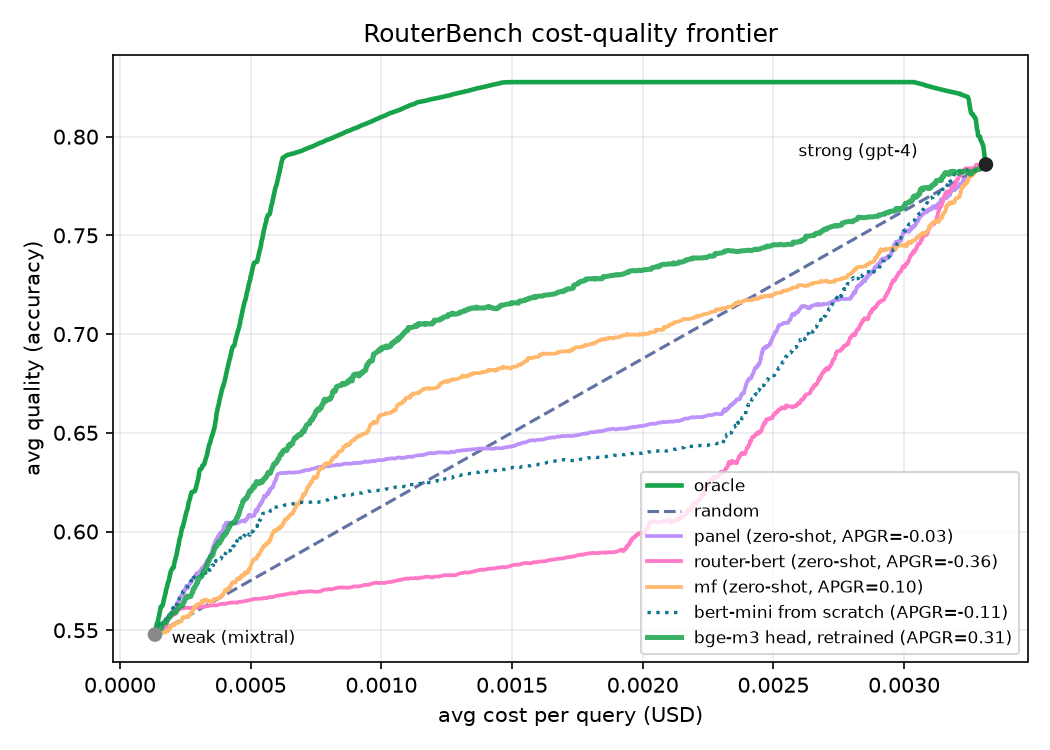
\includegraphics[width=0.86\textwidth]{../../scripts/eval/results/figures/cost_quality.png}
\caption{\rb{} cost-quality frontier. The oracle is the upper envelope; the dashed line
is random mixing. Synthetic-trained routers sit near random; the embedding head trained
on \rb{} climbs toward the oracle.}
\label{fig:cq}
\end{figure}

\subsection{Study 2: the shipped Claude pool --- routing recovers nothing}
The \rb{} weak/strong gap (0.548 vs 0.786) is wide because mixtral and gpt-4 are a
generation apart. The pool LiteForge actually routes over is the Claude family, and there
the tiers are near-parity. On the graded auto-benchmark slices, Claude Haiku reaches
$\sim$95\% of Sonnet's accuracy, and Opus is \emph{Pareto-dominated} (lower measured
accuracy than Sonnet at many times the cost; the oracle selects Opus for under 1\% of
prompts). Running the same binary cost-quality protocol with weak=Haiku, strong=Sonnet,
the embedding head and every baseline land at APGR $\approx 0$ with 95\% CIs that span
zero and overlap each other: there is almost no quality gap to recover, so a learned
router is indistinguishable from defaulting to the cheap tier. The \rb{} headline does
\emph{not} transfer to the shipped pool. This is the paper's pivot: the value is not in
routing the Claude tiers, it is in choosing the right (cheaper) model in the first place.

\subsection{Study 3: cross-provider cost-quality --- where the savings live}
Table~\ref{tab:prov} measures \NPROV{} models on the seven-benchmark pool ($n{=}\NPROMPTS$),
chosen to separate quality rather than saturate it (the gap concentrates in hard
reasoning: GPQA ranges from Sonnet 0.84 down to Mistral 0.38). Three findings:

\paragraph{Cheap hosted models are the cost-quality winners.} DeepSeek v4 Flash reaches
95\% of Sonnet's accuracy at \$0.26/1M (a $\sim$43x unit-cost reduction); Gemini 3.1
Flash-Lite reaches 96\% at \$1.05/1M. Claude Haiku is Pareto-dominated by both. The
cheapest model meeting each quality bar is DeepSeek Flash (\$0.26) at 90\% of Sonnet,
Gemini Flash-Lite (\$1.05) at 95\%, and only Sonnet itself at 99\%.

\paragraph{The open-weight ceiling is $\sim$96\% of Sonnet, and serverless makes it cheap.}
gemma4:31b (0.865), glm-5.2 (0.861), and deepseek-v4-pro (0.854) all land at 95--96\% of
Sonnet, and gpt-oss-120b at 94\%; none beats Sonnet (0.896). On published serverless rates the
strong open-weight models are not just competent but cheap: gemma4:31b serves at \$0.78/1M
(Together), undercutting Gemini Flash-Lite (\$1.05) at marginally higher accuracy, and
gpt-oss-120b at \$0.49/1M (0.844). So the Pareto frontier runs through both cheap hosted models
and serverless open-weight models, and the build-vs-buy question is about residency and control,
not unit cost: renting OSS per-token is already cheap, and owning GPUs only pays at very high,
steady volume. The self-hosted watsonx-class small model (Granite 4.1 8B, 0.735) is
Pareto-dominated by cheaper hosted Mistral Small.

\paragraph{Routing still does not earn its keep here, and build-vs-buy favors hosted.} An
embedding head choosing between the cheap default and Sonnet again returns APGR $0.004$
(95\% CI $[-0.41, 0.39]$): the cheap models are close enough that selection beats routing.
On economics, owning a GPU only beats the cheap hosted frontier above roughly 1B
tokens/month (L40S/H100 amortized), and managed watsonx carries a \$1{,}500--\$5{,}000/month
floor; below serious, steady volume, cheap hosted wins on cost and operational simplicity.

\begin{table}[h]
\centering
\caption{Cross-provider cost-quality, all \NPROV{} models ($n{=}\NPROMPTS$ public-benchmark
prompts; accuracy with 95\% bootstrap CI). Hosted/Claude \$/1M are measured from the gateway;
open-weight (OSS) rows use published serverless rates blended at this token mix (see note). The
two Qwen rows are truncation artifacts (heavy reasoners exceeding the token budget on hard
slices), excluded from conclusions.}
\label{tab:prov}
\scriptsize
\begin{tabular}{@{}llccr@{}}
\toprule
Model & Path & Accuracy (95\% CI) & \% Sonnet & \$/1M \\
\midrule
Sonnet 4.6 & anchor & 0.896 [0.86, 0.93] & 100\% & 11.27 \\
\textbf{gemma4:31b} & OSS & \textbf{0.865 [0.82, 0.90]} & \textbf{96\%} & \textbf{0.78}$^{p}$ \\
glm-5.2 & OSS & 0.861 [0.82, 0.90] & 96\% & 4.08$^{p}$ \\
minimax-m3 & OSS & 0.861 [0.82, 0.90] & 96\% & 1.10$^{p}$ \\
Gemini 3.1 Flash-Lite & hosted & 0.858 [0.82, 0.90] & 96\% & 1.05 \\
deepseek-v4-pro & OSS & 0.854 [0.81, 0.89] & 95\% & 3.31$^{p}$ \\
\textbf{DeepSeek v4 Flash} & hosted & \textbf{0.850 [0.81, 0.89]} & \textbf{95\%} & \textbf{0.26} \\
\textbf{gpt-oss-120b} & OSS & \textbf{0.844 [0.80, 0.89]} & \textbf{94\%} & \textbf{0.49}$^{p}$ \\
qwen3-coder-480b & OSS & 0.841 [0.79, 0.88] & 94\% & 0.79$^{p}$ \\
Haiku 4.5 & anchor & 0.836 [0.79, 0.88] & 93\% & 3.86 \\
devstral-24b & OSS & 0.824 [0.78, 0.87] & 92\% & 0.23$^{p}$ \\
nemotron-ultra & OSS & 0.817 [0.77, 0.86] & 91\% & 3.36$^{p}$ \\
kimi-k2.7 & OSS & 0.817 [0.77, 0.86] & 91\% & 3.87$^{p}$ \\
gpt-oss-20b & OSS & 0.792 [0.75, 0.84] & 88\% & 0.17$^{p}$ \\
gemma3-27b & OSS & 0.771 [0.72, 0.82] & 86\% & 0.14$^{p}$ \\
ministral-14b & OSS & 0.762 [0.71, 0.81] & 85\% & 0.20$^{p}$ \\
nemotron-nano-30b & OSS & 0.761 [0.71, 0.81] & 85\% & 0.19$^{p}$ \\
Mistral Small & hosted & 0.741 [0.69, 0.79] & 83\% & 0.09 \\
Granite 4.1 8B & self-host & 0.735 [0.68, 0.79] & 82\% & 0.19$^{w}$ \\
ministral-8b & OSS & 0.716 [0.67, 0.77] & 80\% & 0.15$^{p}$ \\
ministral-3b & OSS & 0.713 [0.66, 0.77] & 80\% & 0.10$^{p}$ \\
gemma3-12b & OSS & 0.709 [0.65, 0.76] & 79\% & 0.12$^{p}$ \\
qwen3.5 (cloud) & OSS & 0.638$^{\dagger}$ & 71\% & 0.25$^{p}$ \\
gemma3-4b & OSS & 0.620 [0.57, 0.68] & 69\% & 0.09$^{p}$ \\
qwen3.5-397b & OSS & 0.614$^{\dagger}$ & 69\% & 3.47$^{p}$ \\
\bottomrule
\end{tabular}
\\[2pt]
{\footnotesize $^{p}$ published serverless rate (USD/1M) blended at this token mix, fetched
2026-06-27: Together AI for gemma4:31b, glm-5.2, minimax-m3, deepseek-v4-pro, nemotron-ultra,
kimi, gpt-oss-20b/120b, qwen3.5-397b/9b; DeepInfra for qwen3-coder-480b, gemma3-4b/12b/27b,
nemotron-nano-30b; Mistral for ministral-3b/8b/14b and devstral. (This replaces an earlier
owned-compute estimate that was single-stream-throughput noise and inverted the cost ordering.)
$^{w}$ published watsonx Granite price; $^{\dagger}$ truncation artifact, not true quality.}
\end{table}

\begin{figure}[h]
\centering
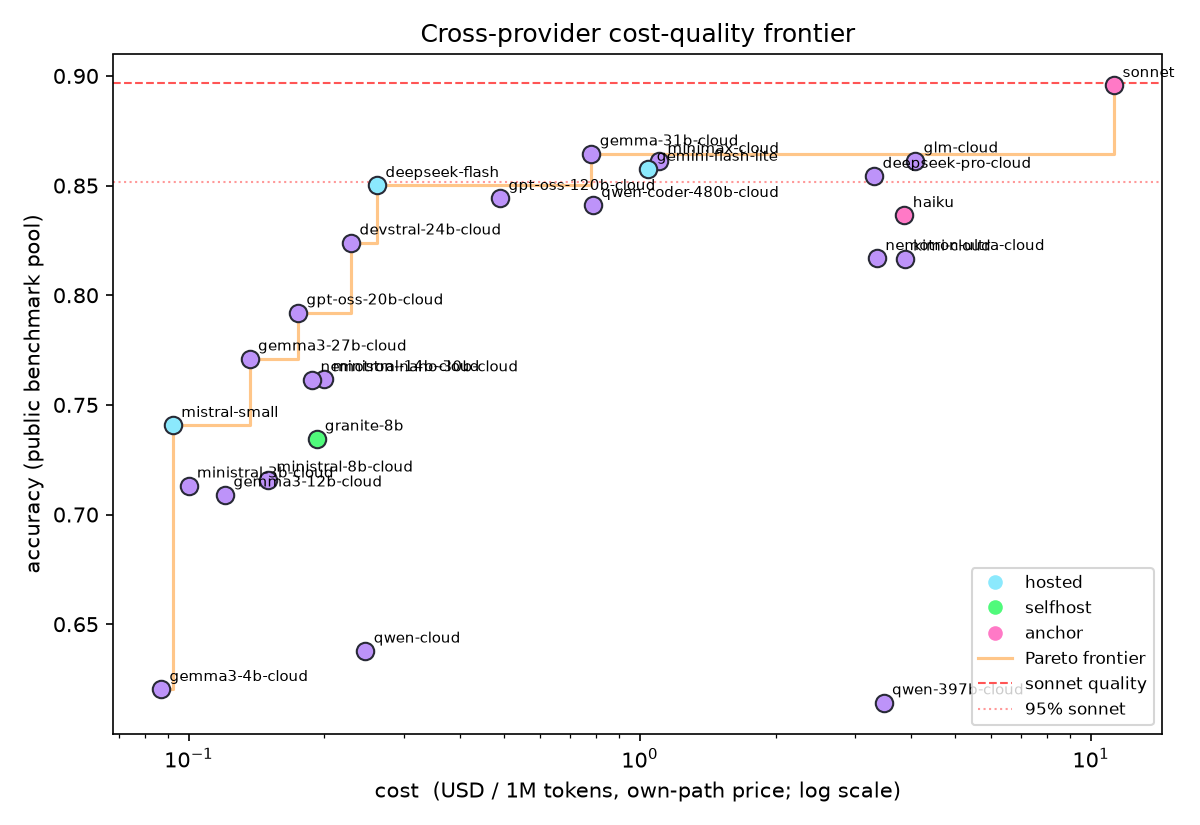
\includegraphics[width=0.86\textwidth]{../../scripts/eval/results/figures/provider_frontier.png}
\caption{Cross-provider cost-quality frontier (accuracy vs \$/1M tokens, log scale). The
Pareto frontier runs through the cheap hosted models; the strong open-weight models match
them on quality but not on cost at this scale, and Claude Haiku sits below the frontier.}
\label{fig:prov}
\end{figure}

\subsection{A methodological note: reasoning-model truncation}
A trap worth flagging: modern reasoning models spend most of their token budget on hidden
thinking before answering, so on hard slices a budget tuned for non-reasoning models
truncates the answer and scores the model as a failure. DeepSeek Flash showed a false 0.30
on GPQA (33/50 responses cut off) until the hard-slice budget was raised, after which its
true accuracy is 0.68; both Qwen cloud models remain truncation artifacts in
Table~\ref{tab:prov} for the same reason. Conversely, an over-generous budget lets a
non-reasoning model run away and (in our case) wedge a shared GPU. Any measured
cost-quality study over a heterogeneous pool must budget per model class and verify
non-empty, parseable answers before trusting a score. The same trap recurs in the agentic
study below: at a 4K budget a reasoning model spent it all on thinking and never emitted its
tool call, producing empty turns that looped to the step cap and scored a false failure
(\code{truncated\_calls} fell from 5 to 0 once raised to 16K); a small LLM judge truncated
before its verdict and silently defaulted to ``escalate.'' Budget per model class and parse an
explicit verdict.

\subsection{Study 4: agentic tasks, where difficulty is illegible up front}
\label{sec:agentic}
The first three studies route on self-contained prompts. Real agents instead run multi-turn,
tool-using episodes whose difficulty only emerges during execution. We test this on
\textbf{tau-bench} (airline, the full \TAUN{}-task test split, real Python tools, a Sonnet-simulated
user, agent temperature 0, 3 trials/task, graded by the environment's database-state reward). The
harness matches the official \code{ToolCallingAgent} (one action per turn, 30-step cap) with full
transcript capture; episodes are cached so strategies are scored offline. Because the OSS tiers are
free via the gateway, the cost axis is a parameter-scaled \$/token proxy applied to measured tokens.

\paragraph{Predictive routing collapses.} The same \code{bge-m3} embedding head, and a
RouteLLM-style port, both score \emph{at or below random} APGR on tau (Table~\ref{tab:agentic}; the
port is significantly negative). The decision signal is the opening user message (``change my
flight''), which does not reveal that the episode requires a one-stop rebooking under a
one-certificate-per-reservation policy. Routing up front is close to blind. This does not contradict
Study~1; it sharpens it: a router is only as valuable as a quality gap it can \emph{see in advance}.

\paragraph{Escalate-on-failure is the frame that works.} Running the cheap tier first and escalating
only when it fails (a cascade) changes the picture. An oracle cascade (escalate iff the cheaper tier
truly failed) reaches \TAUORACLE{} on a weak base and 0.753 on a strong base, both \emph{above}
always-using-the-strongest tier (\TAUSTRONG{}), because it keeps the cheap tier's wins on tasks where
the strong model itself fails. The best cheap, realistic trigger is \emph{self-consistency} (run the
base a few times, escalate on disagreement): 84\% to 98\% of strong quality at $\sim$40--50\% of its
cost, with no verifier.

\paragraph{Verification is the bottleneck.} An LLM-judge cascade depends entirely on the judge: a
strong, calibrated judge (\code{glm-5.2}) reaches recall $\sim$\TAUJUDGEREC{} and the best realistic
quality, but small judges fail in both directions (\code{gemma3:27b} too lenient, recall $\sim$0.05;
\code{qwen3:14b} too harsh), and \emph{none} reach the oracle, because agentic failures are silent:
a wrong booking and a correct one look alike in the transcript, so verifying success is about as
hard as the task. The judge is also the escalation target, so its cost win is small.

\paragraph{The dominant lever is the base model.} Swapping the weak tier from
\code{nemotron-3-nano:30b} to \code{gemma4:31b}, the ``weak'' tier (0.581) \emph{beats} the 397B
``medium'' tier (0.546) at 11x lower cost, and \code{gemma4:31b} alone delivers 93\% of the strongest
tier's quality at 6\% of its cost. As in Studies~2--3, selecting a strong cheap default dominates
clever routing; \code{gemma4:31b} is the same model the cross-provider frontier (Table~\ref{tab:prov})
and the conversational-search study independently pick.

\begin{table}[h]
\centering
\caption{Agentic routing (tau-bench airline, $n{=}\TAUN{}$, 3 trials, param-cost proxy). Quality is
mean DB-state reward; cost is \$/task proxy; \%S is relative to always-strong. Two weak-tier pools.
Predictive routers sit at/below random; cascades dominate; a strong cheap base nearly removes the
need to route.}
\label{tab:agentic}
\scriptsize
\begin{tabular}{@{}lcccc@{}}
\toprule
 & \multicolumn{2}{c}{nemotron base (weak 0.474)} & \multicolumn{2}{c}{gemma base (weak 0.581)} \\
Strategy & Quality & \%S cost & Quality & \%S cost \\
\midrule
all-weak              & 0.474 & 14\% & 0.581 & 6\% \\
all-strong            & 0.628 & 100\% & 0.628 & 100\% \\
predict: router-bert  & 0.573 & 86\% & 0.540 & 87\% \\
predict: mf (APGR $\le$0) & 0.500 & 59\% & --- & --- \\
cascade: give-up      & 0.487 & 67\% & 0.567 & 47\% \\
cascade: self-consistency & 0.526 & 49\% & \textbf{0.613} & \textbf{42\%} \\
cascade: judge (glm-5.2) & 0.600 & 81\% & 0.614 & 55\% \\
cascade: oracle (ceiling) & \textbf{0.727} & 106\% & \textbf{0.753} & 86\% \\
\bottomrule
\end{tabular}
\end{table}

\section{Discussion: when does routing help?}
\label{sec:disc}
The four studies give a clean conditional. Routing pays off only when both a wide
\emph{cost spread} and a \emph{recoverable quality gap} are present \emph{and the gap is
predictable from the input}. \rb{} has all three, and the embedding head recovers 22.5\%. The
Claude pool has the cost spread but not the gap (near-parity tiers), so routing recovers nothing
and the right action is to change the default. The cross-provider pool has an enormous cost
spread, but the cheapest competent models are already 95--96\% as good as the ceiling, so once
again model \emph{selection} on a measured frontier dominates a learned router. Agentic tasks add
the third clause: there the gap is real and wide, but it is \emph{not legible from the opening
turn}, so predictive routing collapses and the answer shifts to \emph{escalate-on-failure}: a
cascade gated by self-consistency (or, where a strong calibrated verifier is justified, an
LLM-judge) recovers most of the headroom, while a strong cheap default (\code{gemma4:31b}) carries
the rest. Across all four, the same lever wins: pick a strong cheap model, then escalate the few
hard cases rather than predict them. We therefore ship the embedding head as an optional selector
but recommend, for near-parity pools, a transparent default-cheap policy with rare escalation, and
for agentic pools an escalate-on-failure cascade rather than an up-front difficulty router.
Limitations: (1) quality in Studies 2--3 is public
benchmarks, directional for real workloads but not a substitute for an in-domain eval;
(2) open-weight \$/1M are published serverless rates (Together/DeepInfra/Mistral) blended at our
token mix, so they track list prices and the chosen provider, not a negotiated contract;
(3) prices are list/homelab, not in-tenant negotiated rates, which shift absolute numbers
but not the shape of the frontier; (4) self-hosting economics (the build-vs-buy break-even) use
single-stream throughput as a proxy and are indicative only; the measured hosted and published
serverless points are the solid frontier; (5) we could not reconcile \rl{}'s released MF (it needs OpenAI
\code{text-embedding-3-small}, unavailable here), so our MF port is retired rather than
defended.

\section{Conclusion}
LiteForge ships a small, native model router with load balancing and a lightweight
embedding-head selector behind an OpenAI-compatible gateway, and we showed honestly when
it helps. On a benchmark with a wide quality gap it recovers a real 22.5\% of cost; on the
near-parity Claude pool it recovers nothing; and across providers the savings come from
\emph{selecting} a cheap competent model (DeepSeek Flash, Gemini Flash-Lite at 95--96\% of
Sonnet for a fraction of the cost), not from routing. The strongest open-weight models
reach $\sim$96\% of Sonnet but are large enough that self-hosting is a high-volume play.
The engineering of a router is sound and reusable; the larger lesson is that on the pools
people actually deploy, disciplined model selection on a measured cost-quality frontier is
the dominant lever, and where a hard tail remains (agentic tasks) the right mechanism is to
escalate on failure, not to predict difficulty up front. Future work: a representative
in-domain eval, in-tenant pricing, completing the open-weight sweep, and a cheap agentic
verifier that can catch silent failures (the current ceiling on cascade quality).

\small
\bibliographystyle{plainnat}
\bibliography{references}

\end{document}
